\section{问题二：2030/2060双碳情景与主体作用}
\subsection{可比情景与目标指标}
为保持同一主体框架下的跨期可比性，本节并列展示问题二的基准推演与问题三的政策强化、供应承压和技术降本情景，后两节继续评价安全风险与投资—运行措施。四情景共享2024年初态与建设结构，GDP增速在2025—2030、2031—2040与其后分别设4.5\%、3.0\%、1.8\%。基准延续工程趋势；政策强化提高碳价漂移、资本和服务效率；供应承压在2030、2045、2060年降低进口和风光水可用出力；技术降本提高资本成本下降速率。

\begin{table}[H]\centering\caption{四情景干预参数}
\begin{tabular}{lrrrr}\toprule
情景 & 碳价漂移/元每吨年 & 年降本/\% & 资本倍率 & 年效率改善/\%\\\midrule
基准延续 & 3 & 1.5 & 1.00 & 0.0 \\
政策强化 & 9 & 2.0 & 1.15 & 0.4 \\
供应承压 & 3 & 1.5 & 1.00 & 0.0 \\
技术降本 & 3 & 4.0 & 1.00 & 0.2 \\
\bottomrule\end{tabular}\end{table}

\begin{figure}[H]\centering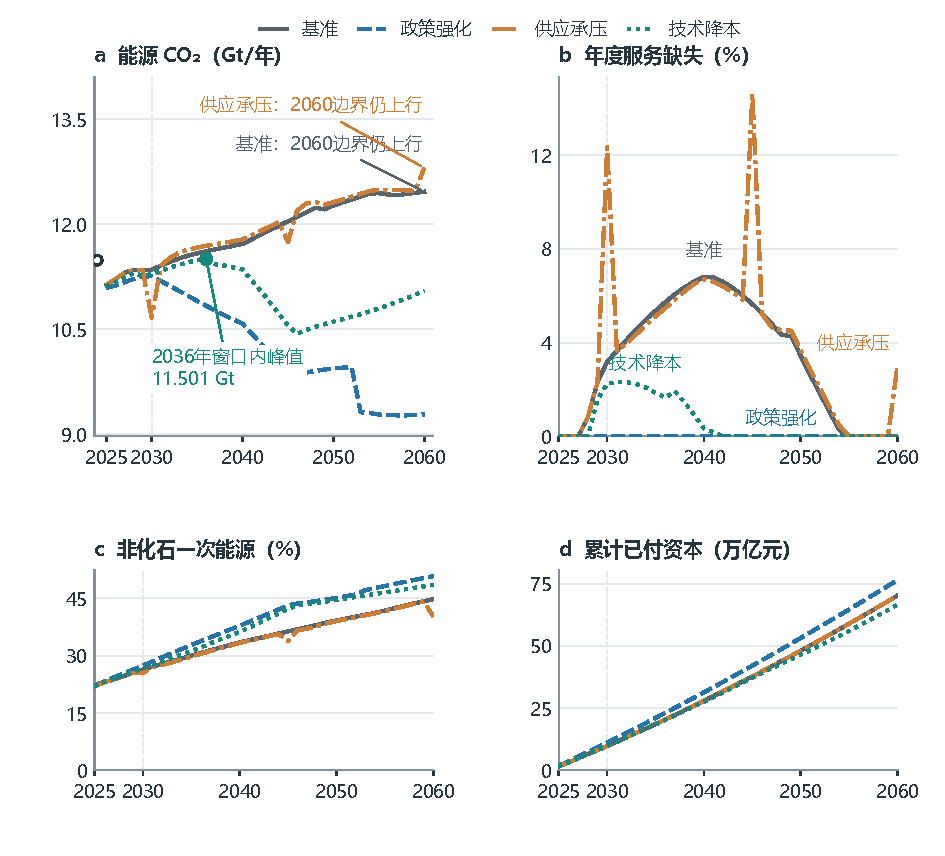
\includegraphics[width=\linewidth]{figures/figA_scenarios.pdf}\caption{终点减排与跨期交付的情景差异。排放与服务缺失为主面板，结构和资本为辅助面板；技术降本情景标注2036年窗口内峰值，末端最大值保留2060边界判定。}\label{fig:figA_scenarios}\end{figure}

\begin{table}[H]\centering\caption{2030/2060能源消费、非化石份额、排放和服务交付}
\begin{tabular}{lrrrr}\toprule
情景/年 & 一次能源/Mtce & 非化石/\% & 能源CO$_2$/Gt & 服务缺失/\%\\\midrule
基准延续/2030 & 6,716 & 26.4 & 11.351 & 3.19 \\
基准延续/2060 & 10,343 & 44.8 & 12.464 & 0.00 \\
政策强化/2030 & 6,732 & 27.4 & 11.259 & 0.00 \\
政策强化/2060 & 9,027 & 50.8 & 9.281 & 0.00 \\
供应承压/2030 & 6,071 & 25.4 & 10.664 & 12.34 \\
供应承压/2060 & 9,909 & 40.4 & 12.807 & 3.09 \\
技术降本/2030 & 6,703 & 26.7 & 11.288 & 2.25 \\
技术降本/2060 & 9,778 & 48.5 & 11.046 & 0.00 \\
\bottomrule\end{tabular}\end{table}

\begin{table}[H]\centering\caption{含2024初态的CO$_2$峰值判定}
\begin{tabular}{lrrrl}\toprule
情景 & 最大年份 & 能源/Gt & 合计/Gt & 判定\\\midrule
基准延续 & 2060 & 12.464 & 13.439 & 窗口末端，尚未确认 \\
政策强化 & 2024 & 11.485 & 12.289 & 初态为窗口最高 \\
供应承压 & 2060 & 12.807 & 13.782 & 窗口末端，尚未确认 \\
技术降本 & 2036 & 11.501 & 12.368 & 窗口内峰值 \\
\bottomrule\end{tabular}\end{table}

\begin{table}[H]\centering\caption{2060强度下降、中和率与剩余净排}
\begin{tabular}{lrrrr}\toprule
情景 & 能源强度降幅/\% & 碳强度降幅/\% & 中和率/\% & 剩余净排/Gt\\\midrule
基准延续 & 30.60 & 56.26 & 5.95 & 12.639 \\
政策强化 & 39.43 & 67.05 & 7.90 & 9.325 \\
供应承压 & 33.51 & 55.15 & 5.80 & 12.982 \\
技术降本 & 34.39 & 61.10 & 6.69 & 11.154 \\
\bottomrule\end{tabular}\end{table}

图\ref{fig:figA_scenarios}显示，技术降本的2036年峰值出现在推演窗口内部，而基准与供应承压直至2060年仍未确认达峰；这使能源结构改善与达峰判定形成不同层次的结果。能源强度以一次能源/GDP计，碳强度以能源加简化工业CO$_2$/GDP计，均相对2024年同口径初态。中和率为固定碳汇除以能源与简化工业总CO$_2$，剩余净排为总量减碳汇；固定碳汇为800 Mt/年。基准与供应承压的最大值出现在2060窗口末端，技术降本在窗口内部达到峰值，政策强化的含初态最高值出现在2024年。各结论对应给定技术和经济条件。
\subsection{多主体交互的涌现机制与条件归因}
保留自主载能趋势，仅关闭政府、消费响应或投资响应，形成四情景完整$2^3$因子实验。消费关闭时沿外生趋势形成份额；另设冻结初始份额的诊断组，考察趋势与响应共同移除的效应。政府关闭仅移除排放误差反馈，投资关闭移除收益和运行响应，所有规则仍接受同一资源约束。

\begin{figure}[H]\centering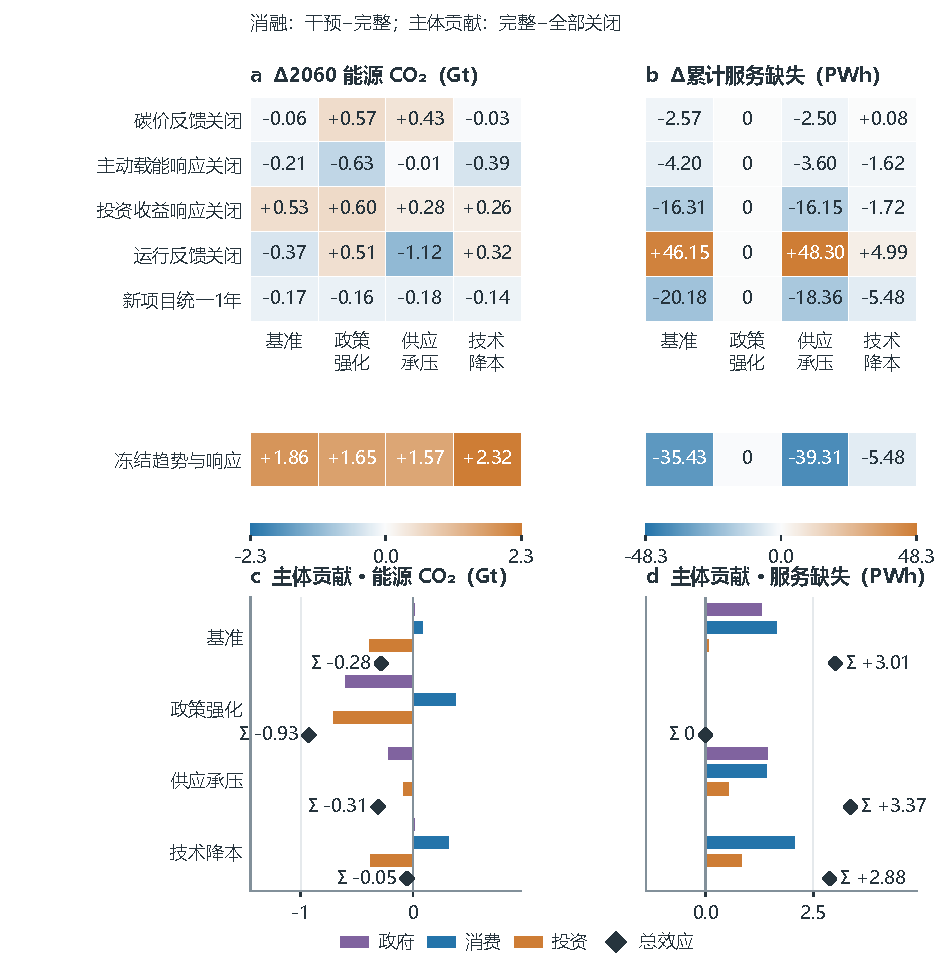
\includegraphics[width=\linewidth]{figures/figB_linked_mechanisms.pdf}\caption{主动主体反馈的减排收益与交付代价。机制反事实差值定义为干预减完整模型；条件Shapley将完整反馈减全关闭的总效应分给三主体。主动载能响应关闭保留趋势，冻结趋势另列诊断；统一一年工期只改变新订单，初始在建队列不变。}\label{fig:figB_linked_mechanisms}\end{figure}

图\ref{fig:figB_linked_mechanisms}揭示减排与交付的跨期权衡：三类主动反馈在基准下合计减少2060年能源CO$_2$ 0.283 Gt，同时增加累计未供有用服务3.011 PWh。政府价格信号、载能选择与资产订单共同作用，需沿建设队列和实际供给解释这一模型内机制结果。

投资响应的Shapley贡献为-385.330 Mt，政府与消费主动响应分别为+14.372与+87.997 Mt，后两者在这一背景下增加排放。冻结初始份额的诊断组对应消费贡献为 -2,460.877 Mt。自主趋势与主动响应对转型结果的贡献需要分开解释。



\begin{figure}[H]\centering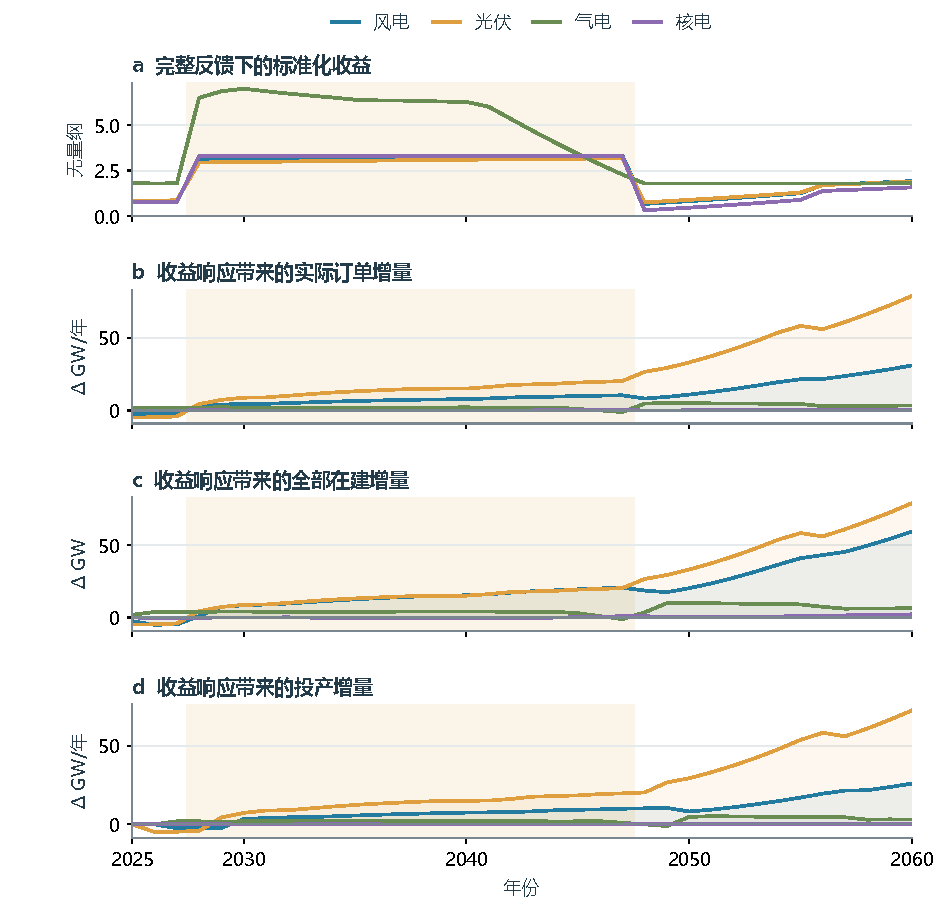
\includegraphics[width=\linewidth]{figures/figB_investment_transmission.pdf}\caption{投资收益响应的传导链。a为完整反馈的标准化收益；b—d为完整反馈减关闭收益响应的订单、全部在建及当年投产差，单位分别为GW/年、GW、GW/年。浅色区为完整反馈电价达到1200元/MWh的2028—2047年；两臂价格、四技术全部原值随表保留。}\label{fig:figB_investment_transmission}\end{figure}
\subsection{联合参数与稀缺定价敏感性}
以固定种子生成48组十维联合工程设计，改变GDP增速、技术成本、降本率、碳价、资本、建设工期、国内供应、进口和行为响应。完整执行每个设计，按排放、服务与资本共同识别敏感区间。稀缺价格另比较800、1200、1600元/MWh阶跃规则及1200元/MWh平滑规则，以检验收益反馈对定价设定的依赖。

\begin{figure}[H]\centering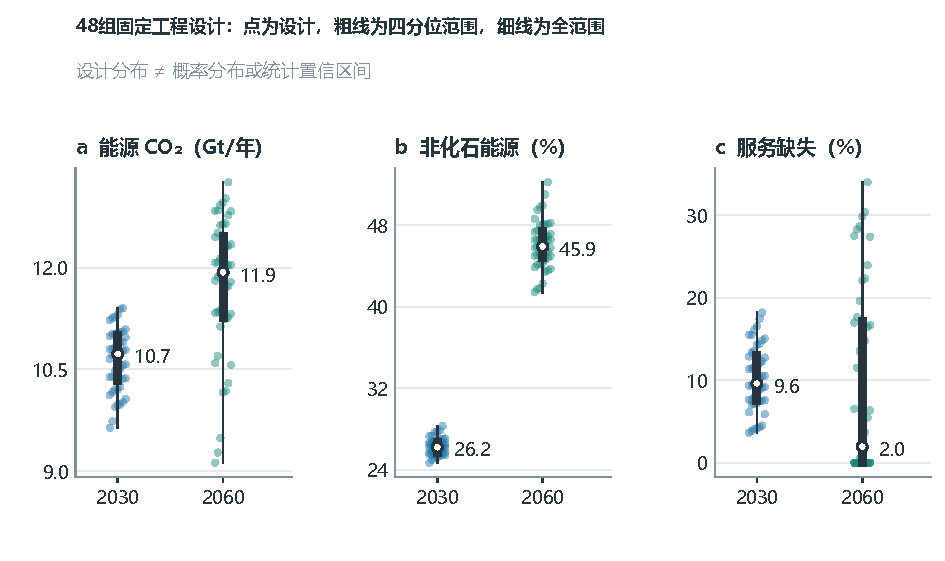
\includegraphics[width=\linewidth]{figures/fig07_joint_design.pdf}\caption{48组联合工程设计的2030与2060离散结果范围。各点为给定设计输出；中位数和极值描述设计集合，不构成概率置信区间。}\label{fig:fig07_joint_design}\end{figure}

\begin{table}[H]\centering\caption{2060年联合设计结果区间}
\begin{tabular}{lrrr}\toprule
指标 & 最小 & 中位 & 最大\\\midrule
能源CO$_2$/Gt & 9.12 & 11.93 & 13.26 \\
非化石/\% & 41.45 & 45.94 & 52.24 \\
服务缺失/\% & 0.00 & 1.95 & 33.98 \\
累计付资/万亿元 & 53.04 & 68.67 & 85.31 \\
\bottomrule\end{tabular}\end{table}

\begin{table}[H]\centering\caption{基准稀缺定价敏感性}
\begin{tabular}{lrr}\toprule
价格规则 & 2060能源CO$_2$/Gt & 累计服务缺失/PWh\\\midrule
阶跃800 & 12.664 & 19.608 \\
阶跃1200 & 12.464 & 35.427 \\
阶跃1600 & 12.411 & 46.642 \\
平滑1200 & 12.648 & 20.687 \\
\bottomrule\end{tabular}\end{table}

\begin{figure}[H]\centering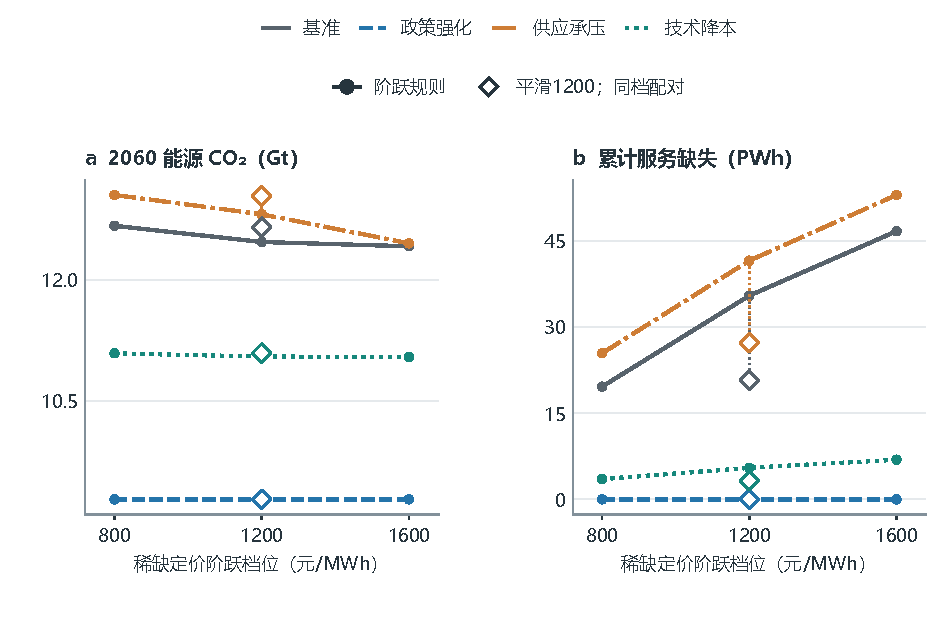
\includegraphics[width=\linewidth]{figures/fig14_price_response.pdf}\caption{稀缺定价的两类干预。阶跃800、1200、1600按数值档位比较，平滑1200以独立标记与阶跃1200配对；函数形状不当作价格数轴延伸。}\label{fig:fig14_price_response}\end{figure}

基准条件下，将稀缺定价阶跃档位由800调整至1200元/MWh，2060年能源CO$_2$由12.664 Gt降至12.464 Gt，而累计未满足服务由19.608 PWh增至35.427 PWh。较强稀缺信号改变利润、订单及后续供给路径，终点排放与跨期交付因此出现不同方向的变化。这是给定工程价格规则下的条件比较，不能直接外推为现实电价变化的数量效应。进口参考折标的敏感性同时保持基年物理留用比例约束；原低档试算因留用比例超过1判为输入不可行，修订后的低档与高档按新协议单独保存。联合工程设计用于比较条件变化。
